\scanpage{44}
\margin{43}
\margin{\unsure{31.11.83|31.12.83}}
\uline{Déploiement} d'un syst. de pseudo-droites. $\underline\Sigma=(X,\Sigma)$, $\Sigma=\unsure{(D_i)_{i\in I}}$

surface compacte $\mathcal X=\mathcal X(\underline\Sigma)$, avec deux sous-graphes $K,L$ tels que $K,L$ découpent cellulairement $\mathcal X$.

a) Tous les pts de $K$ sont d'\uline{ordre 4}. (D'où déploiement $\unsure{\widetilde K'|\widehat K'}$ de $K$ qui est une courbe topologique)

\deleted{\unsure{b)}} Tous les pts de $L$ sont d'ordre pair, les quatre arêtes qui en \unsure{sortent} \inserted{sont distinctes (pas de boucle \unsure{topique})}.

b) \deleted{Pour} toute arête de $K$ contient au plus un sommet de $L$.

c) La réunion \inserted{$K_0$} des adh. des arêtes de $K$ qui ne contiennent pas de sommets \inserted{de $L$ (arêtes exceptionnelles de $K$)} est une réunion finie de cercles, \deleted{indexée par $I$}

\deleted{d) Soit $K_1$ la réunion des autres \unsure{composantes} de}

[Il revient au $=$ d'exiger que \unsure{l'arête} de $K$ \unsure{opposée} à une arête exceptionnelle est exceptionnelle, et que \deleted{\unsure{les pts}}\inserted{\unsure{pour}} les sommets de $K$, il existe au moins une arête issue de ce sommet qui \deleted{n'est pas} est ``ordinaire''.

\deleted{\textcircled{d} \unsure{Alors}} Soit $K_1$ la réunion des adh. des arêtes \deleted{\unsure{exceptionnelles}}\inserted{ordinaires} de sorte que \inserted{$\unsure{\checkmark|N}$} $K'_1$ est une \deleted{réunion de} partie ouverte et fermée \inserted{$\unsure{N}\nearrow$} de $K'$ (i.e réunion de comp. connexes). Alors on \unsure{redonne} une section \deleted{du} fibré des bandes pour l'immersion $K'_1\hookrightarrow\mathcal X$.

\margin{cette donnée résulte en fait des autres, revoir \unsure{position} de e)\quad cf plus bas}

e) Soit $s$ un sommet exceptionnel de $K$ (i.e. sommet incident à une arête exceptionnelle). Alors sur \deleted{\unsure{la}} une arête \inserted{\deleted{\unsure{unique}} non exceptionnelle} \inserted{(pt critique de $K$)} \deleted{iss} incidente à $s$, entre $s$ et le \unsure{1er} sommet de $L$

\figure{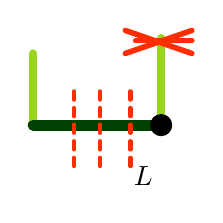
\begin{tikzpicture}[x=.65cm,y=.65cm,line cap=round]
\draw[yellow!60!green,line width=3pt](0,1.4)--(0,0)--(2.5,0)--(2.5,1.7);
\draw[green!25!black,line width=4pt](0,0)--(2.5,0);\fill(2.5,0)circle(4pt);
\draw[red!65!orange,line width=2pt](1.8,1.85)--(3.1,1.4);
\draw[red!65!orange,line width=2pt](1.8,1.4)--(3.1,1.85);
\draw[red!65!orange,line width=2pt](2,1.65)--(3.1,1.65);
\draw[red!65!orange,dashed,line width=1.5pt](.8,-.8)--(.8,.8);
\draw[red!65!orange,dashed,line width=1.5pt](1.3,-.8)--(1.3,.8);
\draw[red!65!orange,dashed,line width=1.5pt](1.9,-.8)--(1.9,.8);
\node at(2.15,-1){$L$};
\end{tikzpicture}}

\inserted{multiplicités des arêtes \inserted{ord} issues de $s$ sont les $=$.}

d'autres pts de $L$. De plus, les \inserted{les deux} deux pts critiques en vis à vis,

f) Pour tt $x\in L\cap K$, ttes branches de $L$ en $x$ croisent les branches de $K$ en $x$. Si $x$ est un sommet de $K$, alors $x$ est un pt d'ordre \deleted{4}\inserted{réduit 2} de $L$. et tout secteur angulaire local de $K$ en $x$ \deleted{\unsure{contient exactement un}} \inserted{\unsure{une arête de} $L$} \inserted{\unsure{deux}} contient exactement une arête de $L$ aboutissant à $x$. (Donc trois cas de figure pour un $x\in K\cap L$

f') Un sommet exceptionnel \inserted{$s$} de $K$ n'est pas sommet de $L$, i.e $s\notin L$.

g) \deleted{Un sommet} Pour un sommet \deleted{ordinaire} $s$ de $K$, pour les 4 arêtes \inserted{(ordinaires)} de $K$ qui en sortent, \unsure{le nb} d'\uline{élts de} $L$ (\deleted{\unsure{prè. de}} entre $s$ et l'unique sommet de $L$ sur l'arête \deleted{\unsure{(point qui est}} indépendant de l'arête, soit $\nu(s)$).

\deleted{Soit $\varepsilon(s)=\left[\begin{array}{ll}+1&\text{si }s\in L\\0&\text{si }s\notin L\end{array}\right.$}

\deleted{Pour ttes arêtes ordinaires, soit $\nu(a)$ la multiplicité réduite de l'unique sommet \unsure{de} $\unsure{-1|L}$}

h) \deleted{Pour tte arête $a$ de $K$, soit $\nu(a)$ le nb des pts simples de $L$ sur $a$ ($=\nu(s)+\nu(s')$, si $a$ est ordinaire d'extrémités $s,s'$) et}

Soit $n$ l'ordre de $\Sigma$. Alors pour tte face $F$ de $K$, le nb des pts de $L$ sur $\partial F$, chacun compté avec sa multiplicité réduite est $2n$.

\margin{NB \unsure{à} $F$ \unsure{ordinaire}, c'est égal :
\[
\sum_{\substack{s\text{ incident}\\\text{à }F}}(2\nu(s)+\varepsilon(s))
+\sum_{\substack{a\text{ incident}\\\text{à }F}}\nu(a)
\]}

\figure{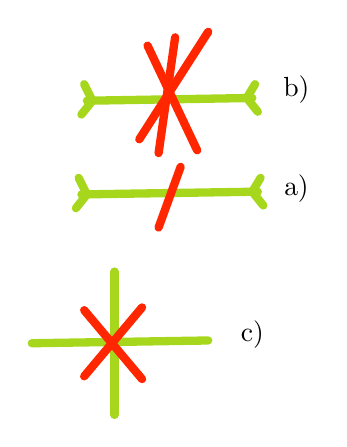
\begin{tikzpicture}[x=.7cm,y=.7cm,line cap=round]
\begin{scope}[shift={(0,4.4)}]
\draw[yellow!65!green,line width=3pt](-1.5,0)--(1.5,.05);
\draw[yellow!65!green,line width=3pt](-1.6,-.25)--(-1.4,0)--(-1.55,.3);\draw[yellow!65!green,line width=3pt](1.6,-.2)--(1.4,.05)--(1.55,.3);
\draw[red!70!orange,line width=3pt](-.4,1)--(.5,-.9);
\draw[red!70!orange,line width=3pt](.1,1.15)--(-.2,-.95);
\draw[red!70!orange,line width=3pt](.7,1.25)--(-.55,-.7);
\node at(2.3,.2){b)};
\end{scope}
\begin{scope}[shift={(0,2.7)}]
\draw[yellow!65!green,line width=3pt](-1.6,0)--(1.6,.05);
\draw[yellow!65!green,line width=3pt](-1.7,-.25)--(-1.5,0)--(-1.65,.3);\draw[yellow!65!green,line width=3pt](1.7,-.2)--(1.5,.05)--(1.65,.3);
\draw[red!70!orange,line width=3pt](.2,.5)--(-.2,-.6);\node at(2.3,.1){a)};
\end{scope}
\begin{scope}
\draw[yellow!65!green,line width=3pt](-2.5,0)--(.7,.05);\draw[yellow!65!green,line width=3pt](-1,1.3)--(-1,-1.3);
\draw[red!70!orange,line width=3pt](-1.55,.6)--(-.5,-.65);\draw[red!70!orange,line width=3pt](-.5,.65)--(-1.55,-.6);\node at(1.5,.15){c)};
\end{scope}
\end{tikzpicture}}

a) $x$ \deleted{\unsure{un sommet de} $L$}\inserted{$\notin S(L)$}, donc pt d'ordre 2 de $L$, alors $x\notin S(K)$

b) $x\in S(L)\cap\mathrm{C}S(K)$

c) $x\in S(L)\cap S(K)$
